
% This LaTeX was auto-generated from an M-file by MATLAB.
% To make changes, update the M-file and republish this document.

\documentclass{article}
\usepackage{graphicx}
\usepackage{color}
\usepackage{listings}
\usepackage[framed]{mcode}
\usepackage{fullpage}
\usepackage{amsmath}
\usepackage[utf8x]{inputenc}
\usepackage{import}
\usepackage{setspace}
\usepackage{hyperref}
\definecolor{lightgray}{gray}{0.5}
\setlength{\parindent}{0pt}

\begin{document}

    
    
%\section*{}


\title{BE 521: Homework 3 Questions\\{\normalsize Feature extraction} \\{\normalsize Spring 2021}}
\author{68 points}
\date{Due: Tuesday, 2/16/2021 10pm}
\maketitle
\textbf{Objective:} Extract features from data and build a simple detector


\begin{center}
\author{Saif Khawaja \\
  \normalsize Collaborators: Raveen K \\}
\end{center}


\section{Features and Simulations (39 pts)} As you learned
in class, features are the backbone of almost all detection
strategies, from seizures in EEG to faces in images. Features are
usually defined in journal articles as an equation or set of
equations, and the task for the reader---if she wants to use that
feature---is to implement that feature in code. In this section, you
will explore and implement some features commonly used in EEG
analysis and test them on simulated time-series data.
\begin{enumerate}
 \item Consider the following toy signal: 7 seconds of a 2 Hz sine
 wave with a quarter period phase-shift, sampled at 100 Hz
  \begin{enumerate}
   \item Plot the signal. (2 pts)

\begin{lstlisting}
frq = 2;

dur = 7;

samp_frq = 100;

tt = 1/samp_frq:(1 / samp_frq):dur;

output = sin(2 * frq * pi * tt - (pi / 2));

figure
plot(tt, output)
xlabel('T (s)')
ylabel('Signal')
title('Toy Signal')
\end{lstlisting}


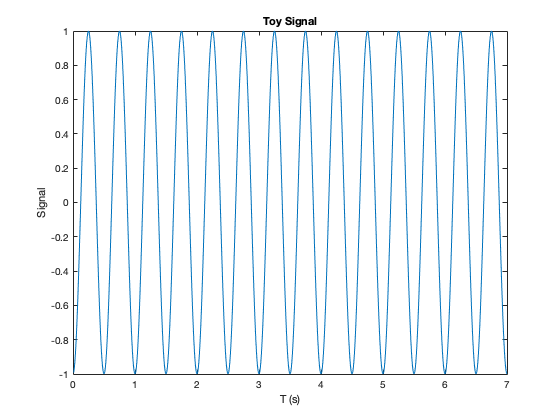
\includegraphics [width=5in]{saif87474921_HW3_01.png}

\item Using the Matlab functions for the difference, sum, and
  absolute value of the elements in a vector (look them up if you
  don't know them), create an anonymous function for the
   line-length feature
	$ LL(\mathbf{x}) = \sum_{i=2}^{n} |x_i - x_{i-1}| $ in one line of
	Matlab code that uses no loops (i.e., the outputs of one function
	will be the inputs of another). Your function should look
	something like \begin{lstlisting}
	  LLFn = @(x) XXXXXX;
	\end{lstlisting}
	where \texttt{XXXXX} represents some use of the aformentioned functions and the input signal \texttt{x}. (4 pts)
   \item What is the line length of this signal? (2 pts)
  \end{enumerate}

\begin{lstlisting}
LLfn = @(x) sum(abs(diff(x)));

LLfn(output)
\end{lstlisting}

\color{lightgray} \begin{lstlisting}
ans =

   55.9921

\end{lstlisting} \color{black}

 \item Consider line length of the signal using a sliding window
 with a certain amount of window overlap (or, to think of it another
 way, displacement with each ``slide''). Now, instead of having just
 one value for the line length, you will have a number of values.
  \begin{enumerate}
	\item Given a signal \texttt{x} with sampling frequency
	\texttt{fs} and windows of length \texttt{winLen} and displacement
	\texttt{winDisp} (both in seconds), create an anonymous function
	called \texttt{NumWins} that calculates the number of possible
	(full) windows in your signal of length \texttt{xLen} (in
	samples), i.e., \begin{lstlisting}
	  NumWins = @(xLen, fs, winLen, winDisp) XXXXXX;
	\end{lstlisting} where \texttt{XXXXXX} is the single-line
	expression for this value. You may assume that \texttt{winDisp} is
	a factor of both \texttt{winLen} (as it usually is/should be)
	and the length (in seconds) of \texttt{x}. (4 pts)

\begin{lstlisting}
NumWins = @(xLen, fs, winLen, winDisp) floor((((xLen/fs) - winLen) / winDisp) + 1);
\end{lstlisting}

  \item Use this
	function to calculate the number of windows for the signal
	described in Question 1.1 for a 400 ms window with 200 ms
	displacement, i.e., the expression \begin{lstlisting}
	  NumWins(length(x), fs, winLen, winDisp)
	\end{lstlisting}
	where \texttt{fs}, \texttt{winLen}, and \texttt{winDisp} are the appropriate values. (1 pt)

\begin{lstlisting}
NumWins(length(output), 100, 0.4, 0.2)

% 33.
\end{lstlisting}

\color{lightgray} \begin{lstlisting}
ans =

    33

\end{lstlisting} \color{black}

	\item Repeat the above calculation for 50 ms window displacement. (1 pt)

\begin{lstlisting}
NumWins(length(output), 100, 0.4, 0.05)

% 132.
\end{lstlisting}

\color{lightgray} \begin{lstlisting}
ans =

   132

\end{lstlisting} \color{black}

	\item Repeat the above calculation for 100 ms window displacement. (1 pt)
  \end{enumerate}

\begin{lstlisting}
NumWins(length(output), 100, 0.4, 0.1)

% 66.
\end{lstlisting}

\color{lightgray} \begin{lstlisting}
ans =

    66

\end{lstlisting} \color{black}

  \item
  \begin{enumerate}
   \item Create a function (in another file) called
   \texttt{MovingWinFeats(x, fs, winLen, winDisp, featFn)} that
   returns a vector of the values of the feature on the signal
   \texttt{x} in all the possible windows, where \texttt{featFn} is
   a feature function like the one you wrote in Question 1.1.b. You
   may find it useful to use your \texttt{NumWins} function (or at
   least its expression). You may assume that the product of
   \texttt{winDisp} and the sampling rate \texttt{fs} is an integer.
   (6 pts) \\


Make sure your MovingWinFeats code is in your pdf. One way is to use the following Matlab code (in your script) to automatically
load in the function's code (where we assume that the function is
one directory up from the *.tex file). Windows users may need to
change the forward-slash to a backslash.

\begin{lstlisting}
%   <latex>
% \lstinputlisting{/Users/saif/Documents/GitHub/braincomputerinterfaces/Homeworks/HW3] MovingWinFeats.m}
%   </latex>
\end{lstlisting}

   \item Using the signal you defined in Question 1.1 and the function you created in Question 1.1.b, calculate the line-length over windows of length 400 ms and displacement 200 ms. (2 pts)

\begin{lstlisting}
% See column.

ans = MovingWinFeats(output, 100, 0.4, 0.2, LLfn)
\end{lstlisting}

\color{lightgray} \begin{lstlisting}
ans =

  Columns 1 through 7

    3.3011    2.8147    2.7652    3.1874    3.5380    3.3011    2.8147

  Columns 8 through 14

    2.7652    3.1874    3.5380    3.3011    2.8147    2.7652    3.1874

  Columns 15 through 21

    3.5380    3.3011    2.8147    2.7652    3.1874    3.5380    3.3011

  Columns 22 through 28

    2.8147    2.7652    3.1874    3.5380    3.3011    2.8147    2.7652

  Columns 29 through 33

    3.1874    3.5380    3.3011    2.8147    2.7652

\end{lstlisting} \color{black}

   \item Add a unit-amplitude 10 Hz signal (in the form of a sine wave) to your original signal and again calculate the line length over the same window and displacement. (2 pts)
  \end{enumerate}

\begin{lstlisting}
% See column.

nfreq = 10;
nsignal = output + sin(2 * pi * tt * nfreq);

feat = MovingWinFeats(nsignal, 100, 0.4, 0.2, LLfn)
\end{lstlisting}

\color{lightgray} \begin{lstlisting}
feat =

  Columns 1 through 7

   15.2595   15.2026   15.2763   15.2140   15.4443   15.2595   15.2026

  Columns 8 through 14

   15.2763   15.2140   15.4443   15.2595   15.2026   15.2763   15.2140

  Columns 15 through 21

   15.4443   15.2595   15.2026   15.2763   15.2140   15.4443   15.2595

  Columns 22 through 28

   15.2026   15.2763   15.2140   15.4443   15.2595   15.2026   15.2763

  Columns 29 through 33

   15.2140   15.4443   15.2595   15.2026   15.2763

\end{lstlisting} \color{black}

  \item Code the following 3 additional features in MINIMAL lines of code (hint: each can be implemented in one line using the anonymous function trick).
  \begin{enumerate}
   \item Area, $\displaystyle A(\mathbf{x}) = \sum_{i=1}^{n} |x_i| $ \quad (2 pts)

\begin{lstlisting}
A = @(x) sum(abs(x))
\end{lstlisting}

\color{lightgray} \begin{lstlisting}
A =

  function_handle with value:

    @(x)sum(abs(x))

\end{lstlisting} \color{black}

   \item Energy, $\displaystyle E(\mathbf{x}) = \sum_{i=1}^{n} x_i^2 $ \quad (2 pts)

\begin{lstlisting}
E = @(x) sum(x.^2)
\end{lstlisting}

\color{lightgray} \begin{lstlisting}
E =

  function_handle with value:

    @(x)sum(x.^2)

\end{lstlisting} \color{black}

   \item Zero-Crossings around mean,\\ $\displaystyle ZX(\mathbf{x}) = \sum_{i=2}^{n} \mathbf{1}(\mathbf{FromAbove}) \;\mbox{OR}\; \mathbf{1}(\mathbf{FromBelow})$,
       where $\mathbf{1}(\cdot)$ denotes the indicator function, which returns a zero if its argument is false and a one if it is true,
       $\mathbf{FromAbove}$ denotes $(x_{i-1} - \overline{x} > 0) \;\mbox{AND}\; (x_i - \overline{x} < 0)$,
       $\mathbf{FromBelow}$ denotes $(x_{i-1} - \overline{x} < 0) \;\mbox{AND}\; (x_i - \overline{x} > 0)$,
       and $\overline{x}$ is the mean value of the elements in $x$. (4 pts)

\begin{lstlisting}
ZX = @(x) sum(abs(diff((x - mean(x)) > 0)))
\end{lstlisting}

\color{lightgray} \begin{lstlisting}
ZX =

  function_handle with value:

    @(x)sum(abs(diff((x-mean(x))>0)))

\end{lstlisting} \color{black}

   \item Plot the values of the four features on the combined signal in the first four cells of a 3x2 matlab subplot.
   Use a 400 ms window with 100 ms displacement. Using the right-aligned convention (where the
   ``official'' time of the feature is that of the last data point
   in the window), give the appropriate time axis for each window
   point. In addition, plot the original signal with the 2Hz and 10Hz
   components in the last two cells of the 3x2 subplot (to make
   comparing down the column easy). Ensure that the time axis in all
   of your plots is the same. (6 pts)

\begin{lstlisting}
t2 = 0.5:0.1:7;

a = MovingWinFeats(nsignal,100,0.4,0.1,A);

l_l = MovingWinFeats(nsignal,100,0.4,0.1,LLfn);

zmc = MovingWinFeats(nsignal,100,0.4,0.1,ZX);

e = MovingWinFeats(nsignal,100,0.4,0.1,E);

figure
subplot(3,2,1)
plot(t2,l_l)
xlabel('T (s)')
ylabel('LL')
title('Line Length')
ylim([15.2 15.45])
xlim([0.5 7])

subplot(3,2,3)
plot(t2,e)
title('Energy')
ylabel('E')
xlabel('T (s)')
xlim([0.5 7])

subplot(3,2,2)
plot(t2, a)
xlabel('T (s)')
ylabel('A')
title('Area')
ylim([30.75 35.75])
xlim([0.5 7])

subplot(3,2,4)
plot(t2,zmc)
xlabel('T (s)')
ylabel('ZMC (Count)')
title('Zero Mean Crossings')
xlim([0.5 7])

subplot(3,2,6)
plot(tt, nsignal)
xlabel('Time (Seconds)')
title('Signal w/ 2Hz and 5Hz Components')
ylabel('S (Units)')
xlim([0 7])

subplot(3,2,5)
plot(tt, nsignal)
xlabel('T (s)')
ylabel('S (Units)')
title('Signal w/ 2Hz and 5Hz Components')
xlim([0 7])
\end{lstlisting}


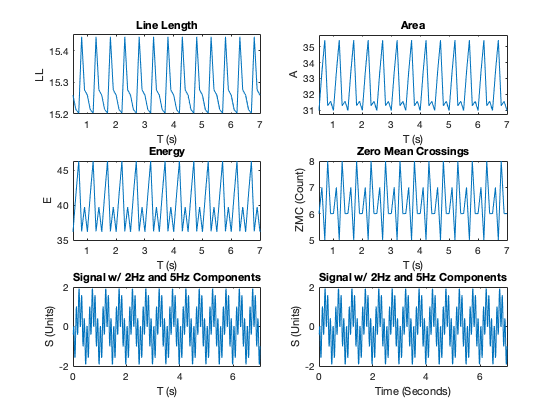
\includegraphics [width=5in]{saif87474921_HW3_02.png}

  \end{enumerate}
\end{enumerate}
\section{Feature Overlays (17 pts)}
In this section, you will use a line-length feature overlay on a segment of EEG containing a seizure. This data is stored in \texttt{I521\_A0003\_D001}
\begin{enumerate}
 \item What is the length using hours:minutes:seconds:milliseconds of the recording? (Use getDuration) (2 pts)

\begin{lstlisting}
session = IEEGSession('I521_A0003_D001', 'saifkhawaja', '/Users/saif/Documents/GitHub/braincomputerinterfaces/Homeworks/sai_ieeglogin.bin' );

durInUSec = (session.data(1).rawChannels(1).get_tsdetails.getDuration);
durInSec = durInUSec / 1e6
durInMin = durInSec/60;

sec = seconds(durInSec);
sec.Format = 'hh:mm:ss.SSS'
\end{lstlisting}

\color{lightgray} \begin{lstlisting}IEEGSETUP: Adding 'ieeg-matlab.jar' to dynamic classpath
Warning: Objects of edu/upenn/cis/db/mefview/services/TimeSeriesDetails class
exist - not clearing java 
Warning: Objects of edu/upenn/cis/db/mefview/services/TimeSeriesInterface class
exist - not clearing java 
IEEGSETUP: Found log4j on Java classpath.
URL: https://www.ieeg.org/services
Client user: saifkhawaja
Client password: ****

durInSec =

   4.8804e+03


sec = 

  duration

   01:21:20.390

\end{lstlisting} \color{black}

 \item How many data points should we discard at the end if we want to clip the recording to the last full second? Do this clipping. (1 pt)

\begin{lstlisting}
nr = ceil((session.data.rawChannels(1).get_tsdetails.getEndTime)/1e6*session.data.sampleRate);
adata = session.data.getvalues(1:nr,1);
session.data

sr = 200;

len = length(adata);

clpd_pnts = (sr / 1000) * (390)
clpd_data = adata(1:(end - clpd_pnts));

% 78.
\end{lstlisting}

\color{lightgray} \begin{lstlisting}
ans = 

  <a href="matlab:help('IEEGDataset')">IEEGDataset</a>:

         snapName: 'I521_A0003_D001'
          montage: As Recorded
           filter: 'No Filter'
         resample: 'Not resampled'
       sampleRate: 200
           values: 
    channelLabels: [1x2 cell]
         annLayer: []
      rawChannels: [1x1 IEEGTimeseries]
      allMontages: [1x44 IEEGMontage]

  <a href="matlab:methods(IEEGDataset)">Methods</a>, <a href="matlab:IEEGObject.openPortalSite()">main.ieeg.org</a>


clpd_pnts =

    78

\end{lstlisting} \color{black}

 \item If we want to overlay a feature trace on the original signal, we have to interpolate that feature (which has been calculated over windows) for each data point of the original signal. One of the simplest methods of doing this is called zero-order interpolation, where we just hold the value constant until we get to the next calculated value. For example, if we had a moving window of 1 second with 1 second displacement, the zero-order interpolated feature vector would have the same value the entire first second, then the same for the entire second second, etc, where each second contains the same number of points as the sampling frequency of the original signal.
 \begin{enumerate}
  \item Using the \texttt{repmat} and \texttt{reshape} functions, create an external function \texttt{zoInterp(x, numInterp} that copies each value of \texttt{x} \texttt{numInterp} times. You can implement this function in one line of code with no loops. Include the code for this function as you did in Question 1.3.a. (2 pts)

\begin{lstlisting}
% <latex>
% \lstinputlisting{/Users/saif/Documents/GitHub/braincomputerinterfaces/Homeworks/HW3] zoInterp.m}
% </latex>
\end{lstlisting}

  \item Confirm that this function works correctly by expanding the length of the vector \texttt{1:5} by a factor of 5 and plotting with the command
  \begin{lstlisting}
	plot(zoInterp(1:5,5),'-o')
  \end{lstlisting}
  where the \texttt{'-o'} option lets us see the individul points as well as the line that connects them. (2 pts)
 \end{enumerate}

\begin{lstlisting}
figure
plot(zoInterp(1:5,5),'-o')
title('zoInterp Expanding 1:5 5 Times')
xlabel('Index')
ylabel('Element')
\end{lstlisting}


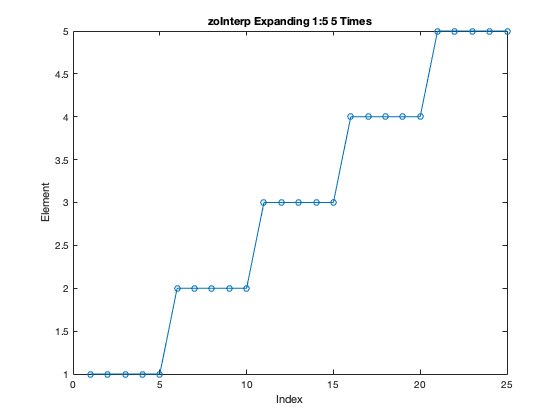
\includegraphics [width=5in]{saif87474921_HW3_03.png}

 \item Using a 5-second sliding window with 1-second displacement,
 calculate the line length feature over the entire signal. Normalize
 the line-length feature values to have a maximum twice that of the
 original EEG signal maximum. Plot the signal in blue and overlay
 the right-aligned line-length feature in yellow. Note: you will need
 to pad your
 signal in order to get them to line up correctly and be the
 same length. Put the units of your time axis in minutes, and be
 sure to add a legend in a location in the plot that does not cover
 up any signal or feature. (6 pts)

\begin{lstlisting}
ll_ns = MovingWinFeats(clpd_data, sr, 5, 1, LLfn);
sf = (2 * max(clpd_data)) / max(ll_ns);

sl = ll_ns * sf;
inter_data = zoInterp(sl, floor(length(clpd_data) / length(ll_ns)));

timed = linspace(1/sr, (length(clpd_data)/sr), length(clpd_data));
timed = timed / 60;

pd = zeros(1, length(clpd_data)-length(inter_data));
pd_data_ft = [pd inter_data];
scaled_padded_data = pd_data_ft * sf;

figure
plot(timed, clpd_data, 'b')
hold on
plot(timed, pd_data_ft, 'y')
xlabel('T (mins)')
ylabel('V (uV)')
legend('Signal', 'LLF', 'Location', 'northwest')
title('I521 A0003 D001 With LLF')
\end{lstlisting}


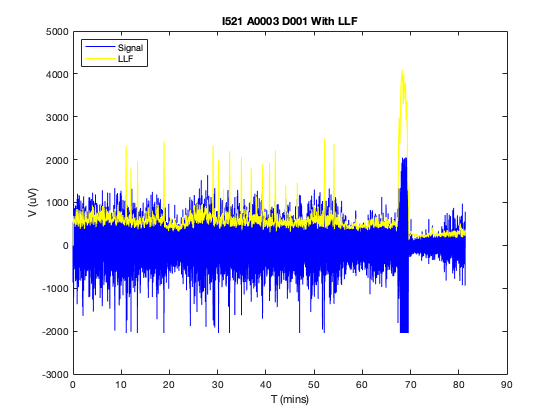
\includegraphics [width=5in]{saif87474921_HW3_04.png}

 \item What threshold might you use on the raw line-length feature
 vector (not the normalized one used for plotting) in order to
 capture the 17 largest pre-seizure chirps that occur? (1 pt)

\begin{lstlisting}
thrsh = 1550 * (1/sf)

% 5.1693x10^4, which works when compared with the data.
\end{lstlisting}

\color{lightgray} \begin{lstlisting}
thrsh =

   5.1693e+04

\end{lstlisting} \color{black}

 \item Using this threshold value, in another plot draw red vertical lines at the leading point in time where the threshold is crossed. Add these vertical lines on top of the plot you made in Question 2.4. These events should capture the pre-seizure chirps, the seizure onset, and some flickering during the end of the seizure. (3 pts)

\begin{lstlisting}
figure
plot(timed, clpd_data, 'b')
hold on
plot(timed, pd_data_ft, 'y')

for k=2:length(pd_data_ft)
    if pd_data_ft(k)> 1550 && pd_data_ft(k-1) < 1550
        xline(timed(k),'r','LineWidth',0.75);
    end
end

xlabel('T (min)')
ylabel('V (uV)')
legend('Signal', 'LLF', 'Crossings', 'Location', 'northeast')
title('Lines Crossing')
xlim([0, 110])
\end{lstlisting}


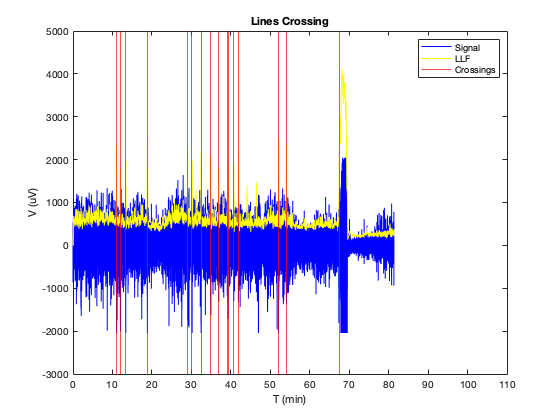
\includegraphics [width=5in]{saif87474921_HW3_05.png}

\end{enumerate}
\section{Building a Detector (12 pts)}
In this section, you will use the features you defined previously to build a seizure detector. Use the EEG data in the file \texttt{I521\_A0003\_D002} with channels \texttt{multiSz\_1}, and \texttt{multiSz\_2}.
\begin{enumerate}
 \item Plot the signal in \texttt{multiSz\_1} and draw vertical red lines at the times when you think the two seizures begin. (You should be able to do this without the need of any features.) (2 pts)

\begin{lstlisting}
session2 = IEEGSession('I521_A0003_D002', 'saifkhawaja', '/Users/saif/Documents/GitHub/braincomputerinterfaces/Homeworks/sai_ieeglogin.bin' );

nr = ceil((session2.data.rawChannels(1).get_tsdetails.getEndTime)/1e6*session2.data.sampleRate);

data2 = session2.data.getvalues(1:nr,1:2);
session2.data;

dur_multiSz_1_uS = session2.data(1).rawChannels(1).get_tsdetails.getDuration;
dur_multiSz_2_uS = session2.data(1).rawChannels(2).get_tsdetails.getDuration;
dur_multiSz_1_S = dur_multiSz_1_uS/1e6;
dur_multiSz_2_S = dur_multiSz_2_uS/1e6;

n_sr = session2.data.sampleRate;

multiSz_1 = data2(:,1);
multiSz_2 = data2(:,2);

t6 = 1/n_sr:1/n_sr:dur_multiSz_1_S+1/n_sr;

figure
plot(t6, multiSz_1)
hold on
xline(7.6, 'r', 'LineWidth', 1.5);
xline(150.2, 'r', 'LineWidth', 1.5);
xlabel('T (min)')
title('MultiSz_1 with Lines for when Two Seizures Start')
legend('Signal', 'Seizure Initialization', 'Location', 'northeast')
ylabel('V (uV)')
\end{lstlisting}

\color{lightgray} \begin{lstlisting}IEEGSETUP: Adding 'ieeg-matlab.jar' to dynamic classpath
Warning: Objects of edu/upenn/cis/db/mefview/services/TimeSeriesDetails class
exist - not clearing java 
Warning: Objects of edu/upenn/cis/db/mefview/services/TimeSeriesInterface class
exist - not clearing java 
IEEGSETUP: Found log4j on Java classpath.
URL: https://www.ieeg.org/services
Client user: saifkhawaja
Client password: ****
\end{lstlisting} \color{black}


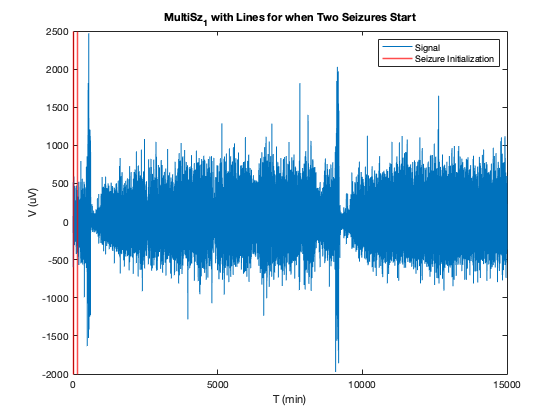
\includegraphics [width=5in]{saif87474921_HW3_06.png}

 \item Produce feature overlay plots similar to that of Question 2.4 for each of the four features you have implemented along with the red vertical lines at each seizure. Use the same 4-second sliding window with 1 second displacement. (4 pts)

\begin{lstlisting}
n_ll = MovingWinFeats(multiSz_1, n_sr, 4, 1, LLfn);
n_a = MovingWinFeats(multiSz_1, n_sr, 4, 1, A);
n_e = MovingWinFeats(multiSz_1, n_sr, 4, 1, E);
n_zmc = MovingWinFeats(multiSz_1,n_sr, 4, 1, ZX);
\end{lstlisting}
\begin{lstlisting}
n_id_length = zoInterp(n_ll, floor(length(multiSz_1) / length(n_ll)));

scaling_factor_ll = (2 * max(multiSz_1))/max(n_id_length);
n_scaled_ll = n_id_length * scaling_factor_ll;

td_new = linspace(1/n_sr, (length(multiSz_1)/n_sr), length(multiSz_1));
td_new = td_new / 60;

pad_ll = zeros(1,length(multiSz_1)-length(n_scaled_ll));

pad_data_ll_n = [pad_ll n_scaled_ll];

figure
plot(td_new, multiSz_1,'b')
hold on
plot(td_new, pad_data_ll_n,'y')
xlabel('T (min)')
ylabel('V (uV)')
title('LLF Overlay MultiSz_1')
xline(7.6, 'r', 'LineWidth', 1.5);
xline(150.2, 'r', 'LineWidth', 1.5);
legend('Signal','LLF', 'Crossings', 'Location', 'northeast')

n_id_area = zoInterp(n_a, floor(length(multiSz_1) / length(n_a)));

sf_a = (2 * max(multiSz_1)) / max(n_id_area);
n_sa = n_id_area * sf_a;

td_new = linspace(1/n_sr,(length(multiSz_1)/n_sr),length(multiSz_1));
td_new = td_new/60;

pad_a = zeros(1, length(multiSz_1) - length(n_sa));

pad_a_n=[pad_a n_sa];

figure
plot(td_new, multiSz_1, 'b')
hold on
plot(td_new, pad_a_n, 'y')
xlabel('T (min)')
ylabel('V (uV)')
title('Area Overlay MultiSz_1')
xline(7.6,'r','LineWidth',1.5);
xline(150.2,'r','LineWidth',1.5);
legend('Signal', 'LLF', 'Crossings', 'Location', 'northeast')

n_id_e = zoInterp(n_e,floor(length(multiSz_1) / length(n_e)));

sf_e = (2 * max(multiSz_1)) / max(n_id_e);
n_s_e = n_id_e * sf_e;

td_new = linspace(1/n_sr,(length(multiSz_1)/n_sr),length(multiSz_1));
td_new = td_new/60;

pad_e = zeros(1,length(multiSz_1)-length(n_s_e));

pad_e_new = [pad_e n_s_e];

figure
plot(td_new,multiSz_1,'b')
hold on
plot(td_new,pad_e_new,'y')
xlabel('T (min)')
ylabel('V (uV)/(uV^2)')
title('Energy Overlay MultiSz_1')
xline(7.6, 'r', 'LineWidth', 1.5);
xline(150.2, 'r', 'LineWidth', 1.5);
legend('Signal', 'Line Length Feature', 'Threshold Crossings', 'Location', 'northeast')

n_id_cross = zoInterp(n_zmc, floor(length(multiSz_1) / length(n_zmc)));

sf_cross = (2 * max(multiSz_1)) / max(n_id_cross);
n_s_cross = n_id_cross*sf_cross;

td_new = linspace(1/n_sr,(length(multiSz_1)/n_sr),length(multiSz_1));
td_new = td_new/60;

pad_cross=zeros(1, length(multiSz_1) - length(n_s_cross));
pad_cross_n = [pad_cross n_s_cross];

figure
plot(td_new,multiSz_1,'b')
hold on
plot(td_new,pad_cross_n, 'y')
xlabel('T (min)')
ylabel('V (uV) // Count')
title('Zero Crossings Around Mean Overlay MultiSz_1')
xline(7.6, 'r', 'LineWidth', 1.5);
xline(150.2, 'r', 'LineWidth', 1.5);
legend('Signal', 'LLF', 'Crossings', 'Location', 'northeast')
\end{lstlisting}


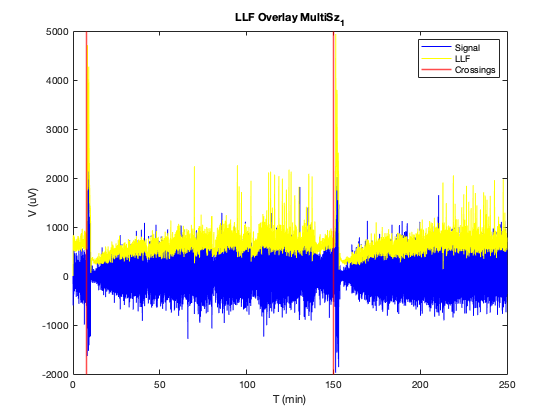
\includegraphics [width=5in]{saif87474921_HW3_07.png}


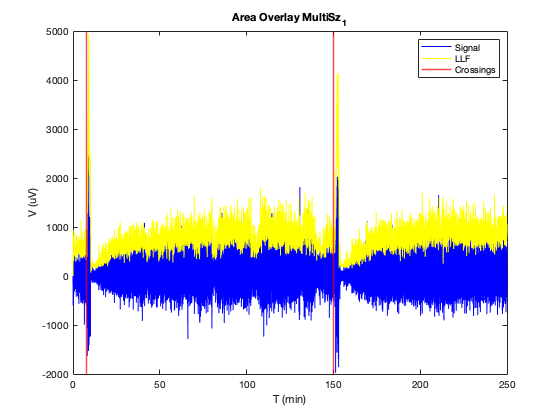
\includegraphics [width=5in]{saif87474921_HW3_08.png}


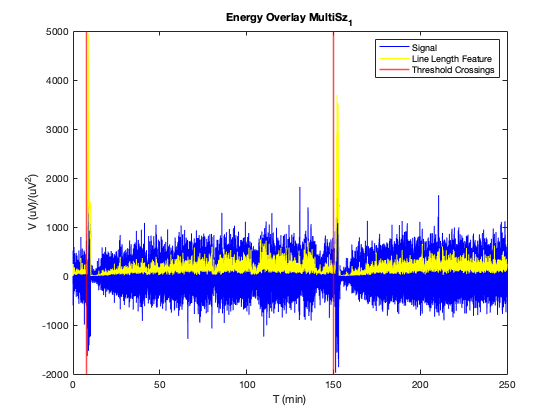
\includegraphics [width=5in]{saif87474921_HW3_09.png}


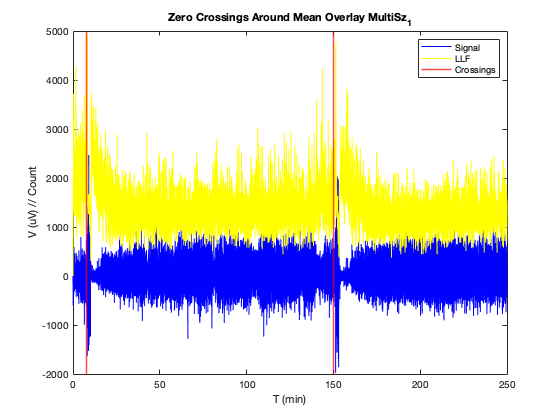
\includegraphics [width=5in]{saif87474921_HW3_10.png}

 \item
  \begin{enumerate}
   \item Based on your plots in the previous question, which of the
   four features seems to give the largest signal (relative to the
   background) for when a seizure occurs? Explain why you think this feature is the best. (3 pts)

\begin{lstlisting}
% Energy seems to be the most successful as the other signals of the
% features generated are smaller relative to the energy plot during
% seizures. The energy therefore has the lowest activity during the
% non-seizure time, but it still spikes during the seizures and we can
% infer a small signal to noise ratio.
\end{lstlisting}

   \item What threshold would you use to determine if a seizure is occurring? (1 pt)

\begin{lstlisting}
thrsh_seiz = 2200*(1/sf_e)

% 1.7582x10^8 uV^2. This is chosen by the energy plot to ignore chirps.
\end{lstlisting}

\color{lightgray} \begin{lstlisting}
thrsh_seiz =

   1.7582e+08

\end{lstlisting} \color{black}

  \end{enumerate}


 \item The signal in \texttt{multiSz\_2} contains another seizure (whose location should again be fairly obvious). Plot the data along with the feature and threshold (horizontal black line, with correct normalization for the signal in \texttt{data2}) you determined in the previous question. (2 pts)

\begin{lstlisting}
e_multiSz2 = MovingWinFeats(multiSz_2,n_sr,4,1,E);

id_e_Sz2 = zoInterp(e_multiSz2,floor(length(multiSz_2)/length(e_multiSz2)));

t_sz2 = t6./60;
tn_sz2 = linspace(1/n_sr,(length(multiSz_2)/n_sr),length(multiSz_2));
tn_sz2 = tn_sz2 / 60;

sf_e_Sz2 = (2 * max(multiSz_2)) / max(id_e_Sz2);
n_s_e_Sz2 = id_e_Sz2 * sf_e_Sz2;

pad_e_Sz2=zeros(1,length(multiSz_2)-length(n_s_e_Sz2));
pad_e_n_Sz2=[pad_e_Sz2 n_s_e_Sz2];

figure
plot(td_new, multiSz_2,'b')
hold on
yline(thrsh_seiz*sf_e,'k','LineWidth',2);
plot(tn_sz2,pad_e_n_Sz2,'y')
xlabel('T (min)')
ylabel('V (uV)//(uV^2)')
title('Energy Overlay MultiSz_2')
legend('Signal', 'Threshold Line', 'Energy', 'Location', 'northeast')
\end{lstlisting}


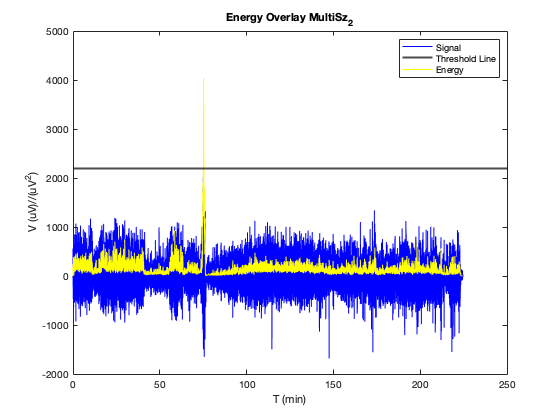
\includegraphics [width=5in]{saif87474921_HW3_11.png}

\end{enumerate}




\end{document}
    
